\section{New Method}

This work aims to find the optimal number and distribution of light cores for a fixed set of cores to achieve the maximum performance-per-watt, with consideration of thermal constraints. In order to estimate the power consumption of a multi-core system for different number of light cores and various light core distributions, we first propose an iteration based full-chip power estimation method with brute force search static, which is accurate but very time-consuming. Furthermore, a non-iteration based method is proposed, which can implement local linearization to avoid time-consuming iterations. Additionally, a greedy based search static can be integrated into the non-iteration based power estimation method to achieve further acceleration.

\subsection{Finding maximum PPW with brute force search static}
As discussed above, the maximum PPW for a multicore chip corresponds to the minimum $P_{1} \times (1-f)+P_{n} \times f/n$, let $P_{a} = P_{1} \times (1-f)+P_{n} \times f/n$ to simplify notation. Noted for dark silicon systems, which are extremely temperature limited, we focus on the major problem of thermal limits, and other constraints can be added with minor modification if needed. The task of finding the maximum PPW can be formulated as the following optimization problem
\begin{equation}
\begin{split}
\text{minimize } & P_{a}\\
\text{subject to} = &\left\{
\begin{array}{c}
T_{c} \preceq T_{th}.\\
\end{array}
\right.
\end{split}
\end{equation}

The optimization problem above is a combinational problem, and its optimal solution can be found by brute force search of all possible combinations of the cores in the multi-core system. Howerver, this brute force search is very computationally expensive. Especially in this case, the number of light core is not set, which means this brute force search static can only be applied to multi-core systems with a small core number. 

\subsection{Iteration based leakage-aware power estimation}
For each of the light cores combination in the optimization problem, we can estimate the power consumption of the multi-core system in series computation process and parallel computation process, with which we could estimate the performance-per-watt of this combination. The steady state power is set by temperature, which is calculated using model (x) by neglecting the differential term $C\frac{dT(t)}{dt}$, leading to
\begin{equation}\label{steady_state_temperature}
T_{c} = L^{T}G^{-1}BP
\end{equation}

It seems straightforward to implement the previous thermal model x for steady state power estimation. By simply providing $P_s(T)$ and $P_d$, we are able to calculate the temperature of each core $T_{c}$. However, such power estimation is valid for dynamic power only scenario and cannot be used when leakage current is considered. This is because $P_{s}(T)$ is a function of current temperature $T_{c}$, leading to the fact that once $T_{c}$ is computed based on $P_{s}(T)$, $P_{s}(T)$ also needs to be updated based on $T_{c}$, which will only stop when steady state is reached.
\begin{figure}
\centering
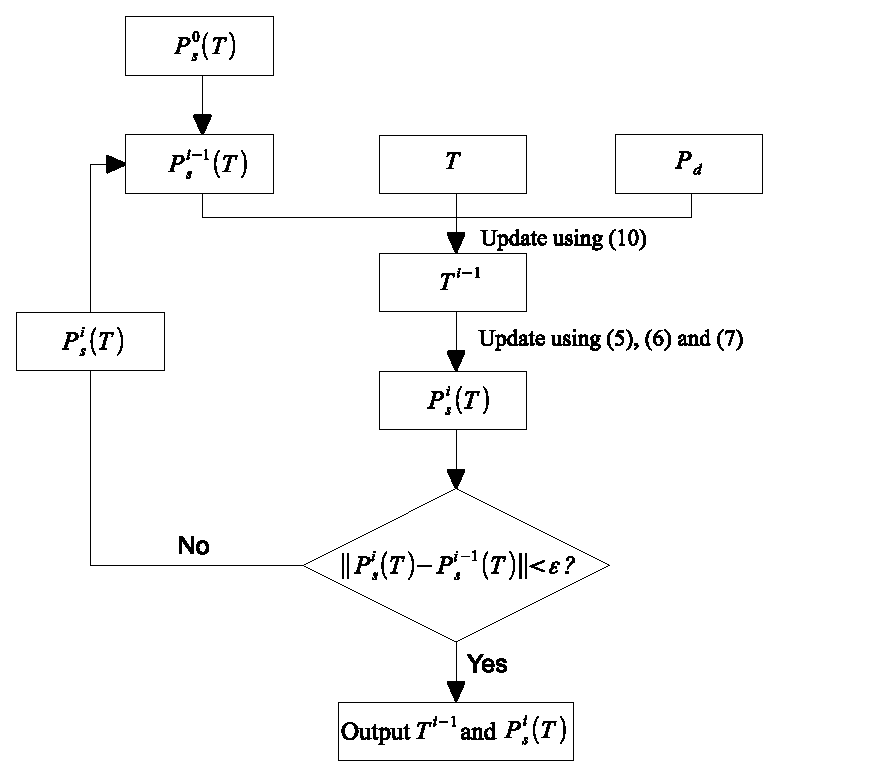
\includegraphics[width=1\linewidth]{fig/iteration_flow.eps}
\caption{Flow diagram of iteration based leakage-aware power estimation for one time step}
\end{figure}

Because of the dependency of static power on temperature, it's not straightforward to compute the static power and temperature of steady state based on current power. Iteration method can be implemented to solve such problem, the computation flow is shown in Fig.x.

The initial value of $P^0_s(T)$ is a guess we provide based on the process technology. The temperature distribution $T^0$ can be calculated with such guess. $P^1_s(T)$, the static power of next time step is updated with $T^0$. Next, the temperature distribution $T^1$ can be derived from $P^1_s(T)$, which concludes one iteration loop. Such iteration goes on until the convergence test is satisfied as $\| P^i_s(T)$-$P^(i-1)_s(T)\|<\epsilon$. Finally, the static power and temperature of steady state is outputted.

Combined with the brute force search static, the iteration based power estimation method can produce an accurate outcome providing the $\epsilon$ is chosen to be small enough, which could be considered as the golden accuracy baseline. However, the simulation time for such iteration based method is way too long, especially for multi-core systems with a large core number. 


\subsection{Local linearized thermal model}
The major difficulty of calculating leakage-aware power estimation comes from the nonlinear thermal model shown in (x), which is caused by the nonlinear relation between subthreshold current and temperature.

To reduce the long computing time caused by iteration method, the leakage current $I_{leak}$ can be linearized to eliminate the non-linearity between $p_{s}$ and temperature, thus accelerating the computation.

Taylor expansion is performed on the original $I_{leak}$ model at a expansion point $T_{0}$. Thus the linearized relation of $I_{leak}$ and temperature is obtained as:
\begin{equation}\label{linear_subthreshold}
\begin{split}
I_{sub} = &K(\frac{k}{q})^{2}e^(\frac{q(V_{GS}-V{th})}{\eta kT_{p0}}\\
&\times (T_{p0}^{2}+(2T_{p0}-\frac{q(V_{GS}-V_{th})}{\eta k})(T_{p}-T_{p0}))\\
&+ o[(T_{p}-T_{p0})^{2}],
\end{split}
\end{equation}
where $o[(T_{p}-T_{p0})^{2}]$ is the remainder. By ignoring the remainder, the linearized $I_{sub}$, denoted as $I_{lin}$ can be expressed as:
\begin{equation}\label{linear_subthreshold}
\begin{split}
I_{lin} = &K(\frac{k}{q})^{2}e^(\frac{q(V_{GS}-V{th})}{\eta kT_{p0}}\\
&\times (T_{p0}^{2}+(2T_{p0}-\frac{q(V_{GS}-V_{th})}{\eta k})(T_{p}-T_{p0})).
\end{split}
\end{equation}

Provided the actual temperature value $T_{p}$ is close to the reference temperature point $T_{p0}$, the approximation accuracy of $I_{lin}$ can be guaranteed. From previous research, it has been shown that due to the characteristic of today's semiconductor process, such local linear approximation of leakage current has high accuracy around the expansion point.

With the linearized relation of subthreshold current and temperature, the relation between static power and temperature in linear form can also be achieved as:
\begin{equation}\label{linear_static}
\begin{split}
p_{s} &= V_{dd}I_{leak}\\
&= V_{dd} \times (I_{lin}+I_{gate})\\
&= V_{dd} \times (I_{lin}(T_{p})+I_{const})
\end{split}
\end{equation}


The linearized static power equation in matrix form is
\begin{equation}\label{linear_static_matrix}
P_{s} = P_{0}+A_{s}T
\end{equation}

\begin{equation}\label{gt=bp}
(G - B_{c}A_{s})T(t) + C\frac{dT(t)}{dt} = B_{c}(P_{d}(t) + P_{0})
\end{equation}

\subsection{Non-iteration based power estimation}
As a property of Taylor expansion approximation, it is accurate only when the actual temperature $T_{p}$ is close to the expansion point $T_{p0}$. As a result, in order to ensure the approximation accuracy, we want each expansion point to be close to the actual temperature $T_{p} in $To find a totally accurate outcome, $T_{p} = T_{p0}$ is necessary. However, such strategy requires $T_{p0}$ to be updated for each iteration, which would lead to longer computing time than we expected. 

However, if we set only one expansion point for all cores with various actual temperature, the approximation accuracy cannot be guranteed.

We can notice that the temperature of cores can be classified into two parts, one is for active-state cores around \SI{70}{\degreeCelsius}, one is for idle-state cores around \SI{40}{\degreeCelsius}. Therefore, in order to balance the accuracy and computing cost, we set two expansion point $T_{p1}$ and $T_{p2}$, one for active cores and another one for idle state cores.


\subsection{Greedy based acceleration of power estimation}
For a multicore chip with $n$ cores, to find the light core number and distribution and determining active core during sequential computation process that leads to the maximum PPW, a ergodic method has to be implemented. The ergodic method is very time-consuming because of the high computational complexity of this problem. 

In previous sections, to find the optimal active core distribution which leads to highest performance-per-watt, for a $n$-core system with different active core numbers,  a combinational method with high complexity is implemented. However, it's  especially impractical when the number of cores is too big. Therefore, a greedy based method which can find a sub-optimal active core distribution with much less time consumption is applied.

For a $n$-core system with $n_{a}$ active cores, the basic idea of finding such sub-optimal solution is described as follows: we first find the optimal solution for only one active core. Next, we fix the first active core position determined by the first step, and find the optimal solution of two cores, with the second active core position determined. Please note that although we say “optimal” in the second step, such solution is only the optimal solution with the first active core fixed at the position determined by the first step, but not the true optimal solution for general two active cores. Similarly, in the ($i$ + 1)-th step, we look for the optimal solution for $i$ + 1 active cores with the positions of $i$ active cores found in all previous steps remain fixed. By proceeding such strategy for $n_{a}$ steps, the sub-optimal solution for $n_{a}$ active cores can be achieved.
